\documentclass[DIV=12,headings=normal]{scrartcl}
\setlength{\parskip}{1em}
\setlength{\parindent}{0pt}

\usepackage[utf8]{inputenc}
\usepackage[T1]{fontenc}
\usepackage[USenglish]{babel}

\usepackage[intlimits]{amsmath}
\usepackage{amssymb}
\usepackage{icomma}
\usepackage{braket}
\usepackage{color}
\usepackage{listings}
\usepackage{hyperref}

\usepackage{graphicx}
%\usepackage{subfig}
\usepackage{booktabs}
\usepackage{pdflscape}
\usepackage{subfigure}

\usepackage{siunitx}
%\sisetup{decimalsymbol=comma}
\usepackage{multirow}
\usepackage{fancyhdr}

\usepackage[version=3,arrows=pgf]{mhchem}

\usepackage{lmodern}
\usepackage{fancyvrb}

\setkomafont{subject}{\usekomafont{title}}
\setkomafont{caption}{\small}
% \captionsetup[subfloat]{font={default,small}}

\newsavebox\MBox
%\newcommand\Cline[2][red]{{\sbox\MBox{#2}%
%  \rlap{\usebox\MBox}\color{#1}\rule[-1.2\dp\MBox]{\wd\MBox}{0.5pt}}}

\newcommand{\comment}[1]{\textcolor{blue}{#1}}
\newcommand{\red}[1]{\textcolor{red}{#1}}
\newcommand{\redl}[1]{{\textcolor{red}{\underline{#1}}}}
\newcommand{\rede}[1]{\redl{#1 <ENTER>}}

\newcommand{\doi}[1]{\href{http://dx.doi.org/#1}{\textcolor{blue}{DOI:~#1}}}
\newcommand{\om}[1]{\omega_{\textrm{#1}}}

\newcommand{\comm}[1]{
\small
~> \redl{#1}
\normalsize
}

\newcommand{\incmo}[1]{\includegraphics[trim=1cm 1cm 1cm 1cm, clip=true, width=4cm]{#1}}
\newcommand{\incom}[1]{\includegraphics[width=3cm]{#1}}

\let\origttfamily=\ttfamily % alte Definition von \ttfamily sichern
\renewcommand{\ttfamily}{\origttfamily \hyphenchar\font=`\-}

\newcommand{\greybox}[1]{
  \vspace{3mm}
  \fcolorbox{black}{black!15}{
    \begin{minipage}{0.9\textwidth}\textit{#1}\end{minipage}}
  \vspace{3mm}
}

\newcommand{\todo}[1]{\textcolor{red}{#1}}

\newcommand{\theo}{\textsc{TheoDORE}}

\newcounter{number}
\newcommand{\numbering}[1]{\thenumber. #1\addtocounter{number}{1}}
\newcommand{\renumber}{\setcounter{number}{1}}

%%%%%%%%%%%%%%%%%%%%%%%%%%%%%%%%%%%%%%%%%%%%%%%%%%%%%%%%%%%%%%%%%%%%%%%%%%%%%%%%%%%%%%%

\fancyhf{}				%Leeren aller Header, Footer
\fancyhead{}		%Links
\fancyfoot[L]{\theo{} tutorial}
\fancyfoot[R]{\thepage}			%Seite x von y
\renewcommand{\headrulewidth}{0pt}	%Linie unter Header

%%%%%%%%%%%%%%%%%%%%%%%%%%%%%%%%%%%%%%%%%%%%%%%%%%%%%%%%%%%%%%%%%%%%%%%%%%%%%%%%%%%%%%%

%\subject{\Large A Tutorial for \theo}
\title{\LARGE A Tutorial for \theo~1.2}
\author{\large Felix~Plasser}
\publishers{\small \textit{Institute for Theoretical Chemistry -- University of Vienna}}
\date{\large Vienna, 2016\\[3em]}

\begin{document}

\pagestyle{fancy}
\selectlanguage{USenglish}

\maketitle
%\cleardoublepage
\vspace{-2em}
\tableofcontents
\clearpage

\section{Before Starting}

\subsection{Introduction}
This tutorial is intended to provide an overview over the functionalities of the \theo{} program package.
Various tasks of different complexity are discussed using interfaces to different quantum chemistry packages.
It is advisable to go through the whole tutorial but it is of course possible to skip some of the later sections.

All input files are contained in the \texttt{EXAMPLES} directory in the \theo{} distribution.
They are the same files accessed by the \texttt{theo\_test.bash} program.

\subsection{Notation}

The following notation is used:

\scriptsize
\begin{Verbatim}[commandchars=\\\{\}]
This kind of font indiates what is seen on the screen
\redl{and the command lines that you should write <ENTER>}  \comment{! Comments come here}
\end{Verbatim}
\normalsize

\greybox{Important information related to \theo{} but not necessarily connected to the current job comes in boxes like this.}

\subsection{Installation}
In case of using \texttt{bash} it should suffice to type

\comm{source /mypath/TheoDORE\_1.2/setpaths.bash} \comment{\scriptsize ! replace /mypath with your actual installation}

to set up the required \texttt{THEODIR}, \texttt{PATH} and \texttt{PYTHONPATH} environment variables.

For more information, see

\url{https://sourceforge.net/p/theodore-qc/wiki/Installation/}

\clearpage
\section{Natural transition orbitals (Turbomole)}

As a first step, we will plot the natural transition orbitals (NTOs) in the case of the formaldehyde dimer computed with RI-CC2 in \textsc{Turbomole}.

\subsection{Input generation}
\label{sec:inpnto}

The input files are taken from the \texttt{EXAMPLES} directory in the \theo{} distribution

\comm{cp -r \$THEODIR/EXAMPLES/fa2.ricc2/QC\_FILES/ fa2.tutorial} \\

Inside the \texttt{fa2.tutorial} directory, run the input program

\comm{theoinp}

\scriptsize
\begin{Verbatim}[commandchars=\\\{\}]
Type of job (rtype):
  [ 1]      qcadc - Q-Chem ADC (libwfa output)
  [ 2]     libwfa - General libwfa output
  [ 3]    qctddft - Q-Chem TDDFT
  [ 4]   colmcscf - Columbus MCSCF
  [ 5]    colmrci - Columbus MR-CI (tden analysis)
  [ 6]      rassi - Molcas RASSI
  [ 7]        nos - Read natural orbitals (Molden format) for sden analysis: Columbus, Molcas, ...
  [ 8]      ricc2 - Turbomole ricc2
  [ 9]       escf - Turbomole escf
  [10]      cclib - Use external cclib library: Gaussian, ORCA, GAMESS, ...
Choice: [8] \redl{8 <ENTER>} \comment{! \texttt{theoinp} tries to guess the program used according to the files present}

Main file to read (rfile):
Choice (autocomplete enabled): [ricc2.out] \redl{<ENTER>}

MO file (Molden format)
 -> This file should ideally contain a square invertible coefficient matrix (mo_file):
Choice (autocomplete enabled): [molden.input] \redl{<ENTER>}

 *** Warning: in the case of ricc2 you have to delete the line
       implicit core=   x virt=    x
     from the control file before running tm2molden.
 \comment{! Everything works here but in general one should remember this when using \texttt{ricc2}}

Analysis of transition density matrices?
Choice (y/n): [y] \redl{<ENTER>}

Perform CT number analysis?
Choice (y/n): [y] \redl{n <ENTER>} \comment{! Do not perform a charge transfer number analysis to keep things simple}

Perform natural transition orbital (NTO) analysis?
Choice (y/n): [y] \redl{<ENTER>}

NTOs as Jmol script? (jmol_orbitals):
Choice (y/n): [y] \redl{y <ENTER>} \comment{! Type "y" if you have the \textsc{Jmol} program available}

NTOs in Molden format (molden_orbitals):
Choice (y/n): [n] \redl{y <ENTER>} \comment{! Type "y" if you want files in \textsc{Molden} format}

Use alpha/beta rather then negative/positive to code for hole/particle orbitals? (alphabeta):
Choice (y/n): [n] \redl{n <ENTER>} \comment{! Only for special applications}

Perform exciton analysis?
Choice (y/n): [y] \redl{n <ENTER>}

Adjust detailed output options?
Choice (y/n): [n] \redl{<ENTER>}

Name of input file
Choice: [dens_ana.in] \redl{<ENTER>}
Finished: File dens_ana.in written.
\end{Verbatim}
\normalsize

After going through these steps, the file \texttt{dens\_ana.in} with the following content is written:

\scriptsize
\begin{Verbatim}[commandchars=\\\{\}]
rtype='ricc2'
rfile='ricc2.out'
mo_file='molden.input'
comp_ntos=True
jmol_orbitals=True
molden_orbitals=True
alphabeta=False
prop_list=['PRNTO']
\end{Verbatim}
\normalsize

\greybox{To learn more about the available keywords check:\\
\url{https://sourceforge.net/p/theodore-qc/wiki/Keywords/}
}


\subsection{Transition density matrix (1TDM) analysis}

To run the 1TDM analysis to produce the NTOs, simply type:

\comm{analyze\_tden.py}

After some technical information, you will find the following output summary

\scriptsize
\begin{Verbatim}[commandchars=\\\{\}]
state       dE(eV)     f  PRNTO \comment{! label of the state / exc. energy / osc. strength / NTO participation ratio}
-------------------------------
1(1)a        4.174 0.000  1.943
2(1)a        4.192 0.000  1.952
3(1)a        7.944 0.000  1.849
4(1)a        8.021 0.164  1.882
5(1)a        8.755 0.000  1.991
6(1)a        8.763 0.052  1.998
\end{Verbatim}
\normalsize


\subsection{Plotting of the orbitals}

If you selected to export files in \textsc{Molden} format, one file for each individual state will be present

\scriptsize
\begin{Verbatim}[commandchars=\\\{\}]
nto_1-1-a.mld  nto_2-1-a.mld  nto_3-1-a.mld  nto_4-1-a.mld  nto_5-1-a.mld  nto_6-1-a.mld
\end{Verbatim}
\normalsize

You can visualize them with any program of your choice.

\clearpage
In the case of using \textsc{Jmol} a shortcut is available.
To plot all the orbitals in one go, simply type

\comm{jmol -n nto\_jmol.spt}

Then \textsc{Jmol} will create \texttt{.png} files for all the orbitals.
To look at all these orbitals at once open the file \texttt{nto.html} in a browser.

\begin{tabular}{|ccl|}
\hline
\textbf{1-1-a} &&\comment{! state label}\\
\comment{! hole/occupied NTO} & \comment{! particle/virtual NTO}&\\
\incmo{fa2/NTO1-1o-56.png} & \incmo{fa2/NTO1-1v-56.png} &\\
0.556 & 0.556 & \comment{! NTO amplitudes $\lambda_i$}\\
\incmo{fa2/NTO1-2o-39.png} & \incmo{fa2/NTO1-2v-39.png} &\\
0.394 & 0.394&\\
\hline
\textbf{2-1-a}&&\\
\incmo{fa2/NTO2-1o-56.png} & \incmo{fa2/NTO2-1v-56.png} &\\
0.556 & 0.556 &\\
\incmo{fa2/NTO2-2o-41.png} & \incmo{fa2/NTO2-2v-41.png} &\\
0.405 & 0.405&\\
\hline
\end{tabular}

\greybox{In both cases two NTO pairs are required to describe the transition, in agreement with $\mathrm{PR_{NTO}}\approx 2$.}\\
\textit{Technical note:} To get the precise pictures shown here, modify the \texttt{nto\_jmol.spt} script
\scriptsize
\begin{Verbatim}[commandchars=\\\{\}]
load molden.input FILTER "nosort"                                                                                                    
mo titleformat "" 
rotate x 90 \comment{! add}
rotate y 10 \comment{! add}
...
\end{Verbatim}
\normalsize

\clearpage

\section{Charge transfer number and exciton analysis (Turbomole)}
In this part an analysis of the charge transfer numbers is carried out.
This requires dividing the system into fragments, which are analyzed together.
Choosing which atoms are grouped into individual fragments and how these fragments are arranged is the first critical step in the charge transfer number analysis. Special care has to be taken when choosing these fragments, and it is often necessary to try different settings.

\subsection{Input generation}
\label{sec:inpct}
First, it is helpful to look at the molecule using a molecular structure editor (e.g. Avogadro) and display the atom lables.

\begin{figure}[h]
\begin{center}
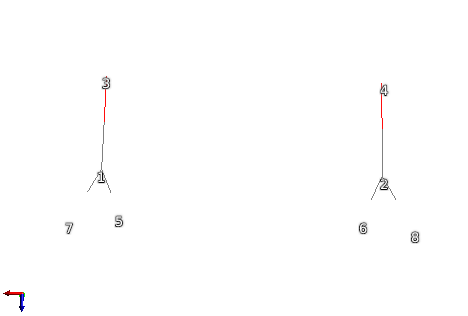
\includegraphics[trim=1cm 2cm 1cm 2cm, clip=true, scale=1]{fa2/fa2avo.png}
\caption{Atom numbering in the formaldehyde dimer.}
\label{fig:fanrs}
\end{center}
\end{figure}

In the present simple case we want to divide our molecule into two fragments, one for each molecule.
One fragment will contain the atom indices 1,3,5,7 the other one 2,4,6,8.

After deciding on the fragment definition run 

\comm{theoinp}

And start out the same as in Section~\ref{sec:inpnto}. Then continue:

\scriptsize
\begin{Verbatim}[commandchars=\\\{\}]
Perform CT number analysis?
Choice (y/n): [y] \redl{y <ENTER>} \comment{! This time we want to do the CT number analysis}

Mode for specifying molecular fragments (at_lists):
  [ 1] Manual input
  [ 2] Automatic generation from coordinate file (using python-openbabel)
  [ 3] Leave empty and fill out later
Choice: \redl{1 <ENTER>} \comment{! We use "Manual input" here, for other options see Section \ref{sec:advinp}}

Input the indices of the atoms belonging to fragment 1:
(separated by spaces)
Choice: \redl{1 3 5 7 <ENTER>} \comment{! Atom indices according to Figure \ref{fig:fanrs}}

Input the indices of the atoms belonging to fragment 2:
(separated by spaces)
Choice: \redl{2 4 6 8 <ENTER>}

Input the indices of the atoms belonging to fragment 3:
(separated by spaces)
Choice:\redl{<ENTER>} \comment{! Leave empty to quit}

Checking whether the at_lists definition is valid ...
at_lists= [[1, 3, 5, 7], [2, 4, 6, 8]]
  2 lists with individual numbers of entries:
[4, 4] \comment{! Two fragments with four atoms each}
  8 total entries, with maximal value 8

Omega descriptors to be computed:
  [ 1] Standard set
  [ 2] Transition metal complex
  [ 3] None
Choice: [1]\redl{<ENTER>}

Print-out of electron/hole populations
  [ 1] None
  [ 2] For fragments
  [ 3] For fragments and individual atoms
Choice: [1]\redl{1 <ENTER>} \comment{! for the symmetric case this analysis does not really help}

Perform natural transition orbital (NTO) analysis?
Choice (y/n): [y]\redl{n <ENTER>} \comment{! already did that before ...}

Perform exciton analysis?
Choice (y/n): [y]\redl{<ENTER>} \comment{! Let's do the exciton analysis here, as well}

Compute approximate exciton size?
Choice (y/n): [y]\redl{<ENTER>}

Molecular coordinates for exciton analysis:
\comment{! for the exciton analysis, it is necessary to have a coordinate file}
Coordinate file (coor_file):
Choice (autocomplete enabled): [coord]\redl{<ENTER>}

Format of coordinate file (coor_format):
Choice: [tmol]\redl{<ENTER>} \comment{! this is the format as recognized by openbabel}
...
\end{Verbatim}
\normalsize
%
\subsection{Transition density matrix (1TDM) analysis}

Again run:

\comm{analyze\_tden.py}

Now, a more extended print-out is available:

\scriptsize
\begin{Verbatim}[commandchars=\\\{\}]
state       dE(eV)     f     Om    POS     PR     CT    COH   CTnt  RMSeh
-------------------------------------------------------------------------
1(1)a        4.174 0.000  0.950  1.500  2.000  0.020  1.041  0.000  1.234
2(1)a        4.192 0.000  0.961  1.500  2.000  0.025  1.052 -0.000  1.245
3(1)a        7.944 0.000  0.971  1.500  2.000  0.175  1.405  0.000  2.362
4(1)a        8.021 0.164  0.968  1.500  2.000  0.207  1.490 -0.000  2.427
5(1)a        8.755 0.000  0.973  1.500  2.000  0.847  1.349 -0.000  3.454
6(1)a        8.763 0.052  0.973  1.500  2.000  0.812  1.440  0.000  3.403
\end{Verbatim}
\normalsize

The meaning of these values is discussed in Refs~\cite{DMAT, DMAT_ADC_II} and at the \href{https://sourceforge.net/p/theodore-qc/wiki/Transition density matrix analysis/}{documentation wiki}. Only a brief explanation shall be given here:

\begin{itemize}
\item
In the case of using \texttt{ricc2} the first value \texttt{Om} or $\Omega$ is just a normalization factor.
In cases, where an exact 1TDM is available, this is the one-electron excitation character.
\item
The values $\om{POS}=1.500$ and $\om{PR}=2.000$ in all cases mean that the excitation is distributed evenly between fragment 1 and fragment 2 (for symmetry reasons)
\item
The crucial information lies in the $\om{CT}$ value. $\om{CT}\approx 0$ for the first four excited states, meaning that these are mostly coupled local excitations (Frenkel excitons). For the last two states $\om{CT}$ is greater than 0.8 indicating that these are charge resonance states.
\item
The trend in the CT values is also reflected by the (approximated) root-mean square electron-hole separation (RMSeh, also denoted $\tilde{d}_{exc}$) given in \AA~\cite{PPV_Steffi}.
This value is is about equal to the intermolecular separation of 3.5~\AA{} in the case of the charge resonance states while it is significantly smaller for the locally excited states.
\end{itemize}

\subsection{Electron-hole correlation plots}
To create electron-hole correlation plots, run

\comm{plot\_OmFrag.py}

Simply use all default values an then look at \texttt{OmFrag.html} in a browser.\\

\begin{tabular}{|cccc|}
\hline
\multicolumn{4}{|l|}{\textbf{Electron-hole correlation plots of the Omega matrices for the}}\\
\multicolumn{4}{|l|}{\textbf{individual states.}}\\
\incom{fa2/pcolor_11a.png}&
\incom{fa2/pcolor_21a.png}&
\incom{fa2/pcolor_31a.png}&
\incom{fa2/pcolor_41a.png}\\
1(1)a & 2(1)a & 3(1)a & 4(1)a\\
\incom{fa2/pcolor_51a.png}&
\incom{fa2/pcolor_61a.png}&
\incom{fa2/axes.png}&
\\
5(1)a & 6(1)a & Axes/Scale & \\
\hline
\end{tabular} \\

Here, the results are rather trivial since there are only two fragments in the calculation, which are equivalent for symmetry reasons.
The locally excited states are represented by black boxes on the main diagonal (going from lower left to upper right) while the charge resonance states are distinguished by off-diagonal contributions.

\section{Interface to the external cclib library (\textsc{Gaussian~09})}
\textsc{Gaussian}, GAMESS, \textsc{Orca}, and some other programs can be parsed through the cclib library, which has to be installed separately.
The present example will also need the \texttt{python-openbabel} package.
If these are available, proceed:

Start by copying the relevant files

\comm{cp -r \$THEODIR/EXAMPLES/fa2.cclib/QC\_FILES/ fa2.cclib.tutorial}

\subsection{Check the log file}
When using cclib, one should start by checking whether the file can be parsed correctly

\comm{cc\_check.py gaussian.log}

\scriptsize
\begin{Verbatim}[commandchars=\\\{\}]
...
Essential attributes:
       mocoeffs ... True
      atombasis ... True
          natom ... True
          homos ... True
     moenergies ... True
     etenergies ... True
         etsyms ... True
         etsecs ... True

Optional attributes:
         etoscs ... True
     aooverlaps ... False
         mosyms ... True

Attributes for structure parsing and creation of Molden file:
         gbasis ... False \comment{! gbasis is missing - no \textsc{Molden} files}
          natom ... True
     atomcoords ... True
        atomnos ... True


 gaussian.log can be parsed by using rtype='cclib' in dens_ana.in.\comment{! this is the important part}
 But conversion to Molden format is not possible
\end{Verbatim}
\normalsize

\subsection{Input generation}
As usual:

\comm{theoinp}

\scriptsize
\begin{Verbatim}[commandchars=\\\{\}]
Type of job (rtype):
  [ 1]      qcadc - Q-Chem ADC (libwfa output)
  [ 2]     libwfa - General libwfa output
  [ 3]    qctddft - Q-Chem TDDFT
  [ 4]   colmcscf - Columbus MCSCF
  [ 5]    colmrci - Columbus MR-CI (tden analysis)
  [ 6]      rassi - Molcas RASSI
  [ 7]        nos - Read natural orbitals (Molden format) for sden analysis: Columbus, Molcas, ...
  [ 8]      ricc2 - Turbomole ricc2
  [ 9]       escf - Turbomole escf
  [10]      cclib - Use external cclib library: Gaussian, ORCA, GAMESS, ...
Choice: \rede{10}

Main file to read (rfile):
Choice (autocomplete enabled): \rede{gaussian.log}

Analysis of transition density matrices?
Choice (y/n): [y]\rede{}

Perform CT number analysis?
Choice (y/n): [y]\rede{}
Fragment definition for CT nubmer analysis

Mode for specifying molecular fragments (at_lists):
  [ 1] Manual input
  [ 2] Automatic generation from coordinate file (using python-openbabel)
  [ 3] Leave empty and fill out later
Choice:\rede{2} \comment{! since there are two well-separated molecules, we can use the automatic mode}

Automatic generation of at_lists partitioning ...

Coordinate file (coor_file):
Choice (autocomplete enabled): \rede{gaussian.log} \comment{! simply take the log file}

Format of coordinate file (coor_format):
Choice: g09 \comment{! format, as recongized by openbabel}
\end{Verbatim}
\normalsize

\greybox{The relevant formats are:\\
\textsc{Gaussian} - g03, g09\\
\textsc{GAMESS} - gamout \\
\textsc{Q-Chem} - qcout}

\scriptsize
\begin{Verbatim}[commandchars=\\\{\}]
*** Fragment composition *** \comment{! Check that everything worked}
  Fragment 1: C H2 O \comment{! This looks reasonable: two formaldehyde molecules}
  Fragment 2: C H2 O

Checking whether the at_lists definition is valid ...
at_lists= [[1, 3, 5, 7], [2, 4, 6, 8]] \comment{! correct indices}
  2 lists with individual numbers of entries:
[4, 4]
  8 total entries, with maximal value 8

Omega descriptors to be computed:
  [ 1] Standard set
  [ 2] Transition metal complex
  [ 3] None
Choice: [1] \rede{}

Print-out of electron/hole populations
  [ 1] None
  [ 2] For fragments
  [ 3] For fragments and individual atoms
Choice: [1] \rede{2}

Perform natural transition orbital (NTO) analysis?
Choice (y/n): [y] \rede{n} \comment{! no possibility to visualize them if \textsc{Molden} export does not work}

Perform exciton analysis?
Choice (y/n): [y] \rede{}

Compute approximate exciton size?
Choice (y/n): [y] \rede{}

Adjust detailed output options?
Choice (y/n): [n] \rede{}

Name of input file
Choice: [dens_ana.in] \rede{}
Finished: File dens_ana.in written.
\end{Verbatim}
\normalsize

The following file \texttt{dens\_ana.in} was created:

\scriptsize
\begin{Verbatim}[commandchars=\\\{\}]
rtype='cclib'
rfile='gaussian.log'
coor_file='gaussian.log'
coor_format='g09'
at_lists=[[1, 3, 5, 7], [2, 4, 6, 8]]
eh_pop=1
comp_ntos=False
prop_list=['Om', 'POS', 'PR', 'CT', 'COH', 'CTnt', 'RMSeh']
\end{Verbatim}
\normalsize

\subsection{Transition density matrix (1TDM) analysis}
Again run:

\comm{analyze\_tden.py}

The output looks similar as it did before only that at the TDDFT/PBE level the CT states are lower in energy.

\scriptsize
\begin{Verbatim}[commandchars=\\\{\}]
state       dE(eV)     f     Om    POS     PR     CT    COH   CTnt  RMSeh
-------------------------------------------------------------------------
Singlet-A2   3.583 0.000  1.000  1.500  2.000  0.698  1.729  0.000  3.179
Singlet-B1   3.635 0.000  1.000  1.500  2.000  0.737  1.633  0.000  3.257
Singlet-B1   4.242 0.000  1.001  1.500  2.000  0.262  1.632  0.000  2.141
Singlet-A2   4.284 0.000  1.001  1.500  2.000  0.301  1.727 -0.000  2.256
Singlet-B2   7.793 0.011  1.001  1.500  2.000  0.958  1.088  0.000  3.656
Singlet-A1   7.851 0.001  1.000  1.500  2.000  0.992  1.015  0.000  3.717
...
\end{Verbatim}
\normalsize

\clearpage
\section{Advanced fragment input and double excitations (Columbus)}
\label{sec:advinp}

The secure way for fragment definition is always the manual mode described in Section~\ref{sec:inpnto}.
In some cases, i.e. when the fragments of interest are separate molecules, one can use the option "Automatic generation from coordinate file" in \texttt{theoinp}.
A more involved method for automatic fragment definition is described in the next section.
This method relies on the \textsc{Avogadro} molecular structure editor and the availability of the \texttt{python-openbabel} package.

This method is described in the next two sections.
If you just wish to run the job without the input generation, copy the \texttt{dens\_ana.in file} given at the bottom of Section~\ref{sec:inpcol}.

Take the input files from the \texttt{EXAMPLES} directory in the \theo{} distribution

\comm{cp -r \$THEODIR/EXAMPLES/hexatriene.colmrci/QC\_FILES/ hexatriene.tutorial} \\


\clearpage
\subsection{Fragment preparation using Avogadro}

First the \texttt{geom} file in \textsc{Columbus} format has to be converted to the more common xyz format.

\comm{babel.py col geom xyz geom.xyz}

\greybox{This step is specific for \textsc{Columbus}. In many other cases \textsc{Avogadro} can directly read the structure file or logfile.}

This file can be opened with \textsc{Avogadro}

\comm{avogadro geom.xyz}

In \textsc{Avogadro} the following steps have to be performed (Figure~\ref{fig:avo})

\begin{enumerate}
\item
Click the pen (draw tool)
\item
Uncheck "Adjust Hydrogens"
\item
Right-click the bonds that you wish to delete to divide the molecule into fragments
\item
Save the file as \texttt{geom.mol} \comment{! use a structure format with explicit bonds}
\end{enumerate}

\begin{figure}[h!]
\begin{center}
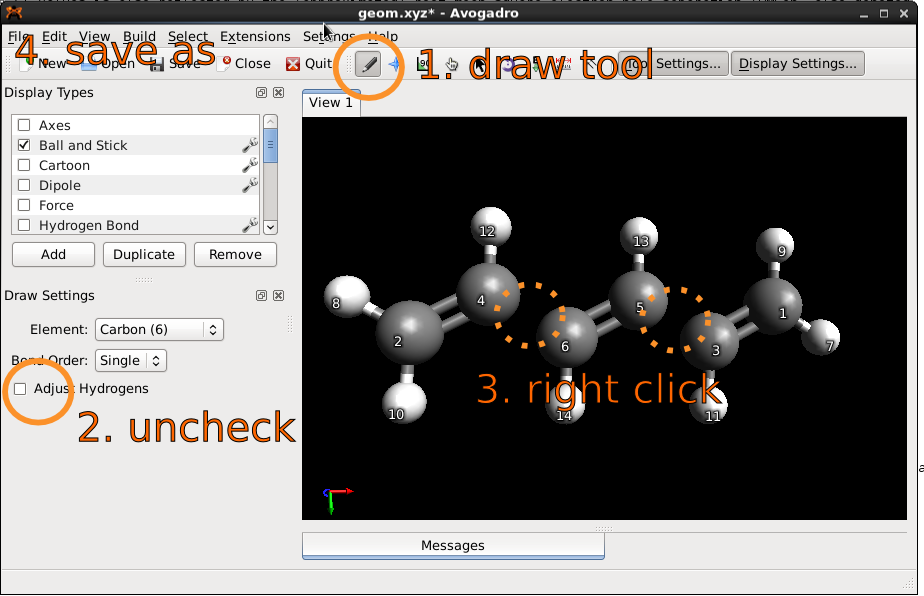
\includegraphics[trim=0cm 0cm 0.1cm 0cm, clip=true, scale=0.5]{avo_instructions.png}
\caption{Fragment definition using \textsc{Avogadro}.}
\label{fig:avo}
\end{center}
\end{figure}

\subsection{Input generation}
\label{sec:inpcol}
Now run \texttt{theoinp} using the newly created \texttt{geom.mol} file as a template.

\comm{theoinp}

\scriptsize
\begin{Verbatim}[commandchars=\\\{\}]
Type of job (rtype):
  [ 1]      qcadc - Q-Chem ADC (libwfa output)
  [ 2]     libwfa - General libwfa output
  [ 3]    qctddft - Q-Chem TDDFT
  [ 4]   colmcscf - Columbus MCSCF
  [ 5]    colmrci - Columbus MR-CI (tden analysis)
  [ 6]      rassi - Molcas RASSI
  [ 7]        nos - Read natural orbitals (Molden format) for sden analysis: Columbus, Molcas, ...
  [ 8]      ricc2 - Turbomole ricc2
  [ 9]       escf - Turbomole escf
  [10]      cclib - Use external cclib library: Gaussian, ORCA, GAMESS, ...
Choice: [5] \rede{}

MO file (Molden format)
 -> This file should ideally contain a square invertible coefficient matrix (mo_file):
Choice (autocomplete enabled): [MOLDEN/molden_mo_mc.sp] \rede{}

Analysis of transition density matrices?
Choice (y/n): [y] \rede{}

Perform CT number analysis?
Choice (y/n): [y] \rede{y}
Fragment definition for CT nubmer analysis

Mode for specifying molecular fragments (at_lists):
  [ 1] Manual input
  [ 2] Automatic generation from coordinate file (using python-openbabel)
  [ 3] Leave empty and fill out later
Choice: \rede{2} \comment{! use automatic generation if python-openbabel is available}
Automatic generation of at_lists partitioning ...

Coordinate file (coor_file):
Choice (autocomplete enabled): [geom] \rede{geom.mol} \comment{! specify the newly created file}

Format of coordinate file (coor_format):
Choice: [col] \rede{mol}

*** Fragment composition ***
  Fragment 1: C2 H3
  Fragment 2: C2 H3
  Fragment 3: C2 H2 \comment{! the central \ce{C2H2} fragment is at the end ...}
\comment{  ! ... his has to be changed (see below)}
Checking whether the at_lists definition is valid ...
at_lists= [[1, 3, 7, 9, 11], [2, 4, 8, 10, 12], [5, 6, 13, 14]]
  3 lists with individual numbers of entries:
[5, 5, 4]
  14 total entries, with maximal value 14

Omega descriptors to be computed:
  [ 1] Standard set
  [ 2] Transition metal complex
  [ 3] None
Choice: [1] \rede{}

Print-out of electron/hole populations
  [ 1] None
  [ 2] For fragments
  [ 3] For fragments and individual atoms
Choice: [1] \rede{2}

Perform natural transition orbital (NTO) analysis?
Choice (y/n): [y] \rede{n}

Perform exciton analysis?
Choice (y/n): [y] \rede{n}

Were there frozen core orbitals in the calculation?
Choice (y/n): [y] \rede{n} \comment{! for general \textsc{Columbus} jobs frozen core orbitals would have to be specified here}

Adjust detailed output options?
Choice (y/n): [n] \rede{}

Name of input file
Choice: [dens_ana.in] \rede{}
Finished: File dens_ana.in written.
\end{Verbatim}
\normalsize

In the \texttt{dens\_ana.in} file, it is necessary to adjust the fragment definitions in \texttt{at\_lists} to make sure that the central \ce{C2H2} fragment is really in the middle.
The file should look like this:

\scriptsize
\begin{Verbatim}[commandchars=\\\{\}]
rtype='colmrci'
mo_file='MOLDEN/molden_mo_mc.sp'
coor_file='geom.mol'
coor_format='mol'
at_lists=[[1, 3, 7, 9, 11], [5, 6, 13, 14], [2, 4, 8, 10, 12]] \comment{! this was adjusted manually}
eh_pop=1
comp_ntos=False
prop_list=['Om', 'POS', 'PR', 'CT', 'COH', 'CTnt']
\end{Verbatim}
\normalsize
\vspace{-1em}
\greybox{When using the automatic fragment definition, it is generally advisable to check the results using a graphical representation of the molecule (c.f. Figure~\ref{fig:avo}) and to adjust things if necessary.}
\vspace{-1.5em}
\subsection{Transition density matrix (1TDM) analysis}
\vspace{-1em}
As always:
\comm{analyze\_tden.py}
\vspace{-0.5em}
\scriptsize
\begin{Verbatim}[commandchars=\\\{\}]
Decomposition over fragments
I1.1-2
-------------------------------------------------------
       Fragment        h+        e-       sum      diff
-------------------------------------------------------
         C2 H3    0.12017   0.11046   0.23063   0.00972
         C2 H2    0.13515   0.15458   0.28973  -0.01944
         C2 H3    0.12017   0.11046   0.23063   0.00972
-------------------------------------------------------
                  0.37549   0.37549   0.75099  -0.00000
-------------------------------------------------------

...

state       dE(eV)     f     Om    POS     PR     CT    COH   CTnt
------------------------------------------------------------------
I1.1-2       5.565 0.000  0.375  2.000  2.955  0.823  2.670  0.000
I2.1-1       6.530 1.254  0.865  2.000  2.885  0.613  2.845  0.000
I2.1-2       6.772 0.006  0.432  2.000  2.838  0.938  1.641  0.000
\end{Verbatim}
\normalsize

\greybox{The first and third states show predominant double excitation character $(\Omega<0.5)$.
Note, that in these cases the 1TDM analysis does not provide a complete description.}

\section{Attachment/detachment analysis (Molcas - natural orbitals)}
While the previous examples were focused on an analysis of the transition density matrices, TheoDORE can also analyze state- and difference-density matrices.
These are most conveniently read in as natural orbital (NO) files in \textsc{Molden} format.

\subsection{Input generation}
Get the input files \\
\comm{cp -r \$THEODIR/EXAMPLES/fa2.rassi/QC\_FILES/ fa2.rassi.tutorial}

and call \comm{theoinp}

\scriptsize
\begin{Verbatim}[commandchars=\\\{\}]
Type of job (rtype):
  [ 1]      qcadc - Q-Chem ADC (libwfa output)
  [ 2]     libwfa - General libwfa output     
  [ 3]    qctddft - Q-Chem TDDFT              
  [ 4]   colmcscf - Columbus MCSCF
  [ 5]    colmrci - Columbus MR-CI (tden analysis)
  [ 6]      rassi - Molcas RASSI
  [ 7]        nos - Read natural orbitals (Molden format) for sden analysis: Columbus, Molcas, ...
  [ 8]      ricc2 - Turbomole ricc2
  [ 9]       escf - Turbomole escf
  [10]      cclib - Use external cclib library: Gaussian, ORCA, GAMESS, ...
Choice: [6] \rede{7} \comment{! let's use the generic NO interface here}

MO file (Molden format)
 -> This file should ideally contain a square invertible coefficient matrix (mo_file):
Choice (autocomplete enabled): \rede{molcas.rasscf.molden}

Directory with the NO files:
Choice (autocomplete enabled): [.] \rede{}
. contains the following files:
  [ 1] MOLCAS.input
  [ 2] MOLDEN.1
  [ 3] MOLDEN.2
  [ 4] MOLDEN.3
  [ 5] TRD
  [ 6] geom.xyz
  [ 7] molcas.log
  [ 8] molcas.rasscf.molden

Input indices of required files (separated by spaces)
 Start with ground state.
Choice: \rede{2 3 4} \comment{! we want to analyze the files MOLDEN.1, MOLDEN.2, MOLDEN.3}

Analysis of state density matrices?
Choice (y/n): [y] \rede{}

Print out Mulliken populations? (pop_ana):
Choice (y/n): [y] \rede{}

Compute number of unpaired electrons? (unpaired_ana):
Choice (y/n): [y]  \rede{n} \comment{! this does not currently work in the case of spin-NOs as used by Molcas}

Attachment/detachment analysis (AD_ana):
Choice (y/n): [y] \rede{y}

NDOs as Jmol script? (jmol_orbitals):
Choice (y/n): [y] \rede{}

NDOs in Molden format? (molden_orbitals):
Choice (y/n): [n] \rede{}

Mayer bond order and valence analysis? (BO_ana):
Choice (y/n): [y] \rede{}

Adjust detailed output options?
Choice (y/n): [n] \rede{}

Name of input file
Choice: [dens_ana.in] \rede{}
Finished: File dens_ana.in written.
\end{Verbatim}
\normalsize

\subsection{State density matrix analysis}
This time, we run the program

\comm{analyze\_sden.py}

\scriptsize
\begin{Verbatim}[commandchars=\\\{\}]
Mulliken populations \comment{! ground state}
MOLDEN.1            
----------------    
  Atom     state    
----------------    
  C  1   5.92413    
  C  2   5.92413    
  O  3   8.35389    
  O  4   8.35389    
  H  5   0.86099    
  H  6   0.86099    
  H  7   0.86099    
  H  8   0.86099    
----------------    
        32.00002    
----------------    

MOLDEN.2 \comment{! first excited state}
------------------------------------
  Atom     state       det       att
------------------------------------
  C  1   6.04465   0.03847  -0.15898 \comment{! detachment/attachment with respect to ground state}
  C  2   6.04465   0.03847  -0.15898
  O  3   8.28628   0.45914  -0.39152
  O  4   8.28628   0.45914  -0.39152
  H  5   0.83454   0.02650  -0.00004
  H  6   0.83454   0.02650  -0.00004
  H  7   0.83454   0.02650  -0.00004
  H  8   0.83454   0.02650  -0.00004
------------------------------------
        32.00000   1.10119  -1.10117 \comment{! sum: promotion number \textit{p}}
------------------------------------

...

Valence information \comment{! valence analysis from Ref. \cite{Mayer_BO}}
 Total valence (V\_A)
 Free valence (F\_A) 
MOLDEN.1            
--------------------------
  Atom       V\_A       F\_A
--------------------------
  C  1   3.67354   0.19140
  C  2   3.67354   0.19140
  O  3   1.85728   0.19063
  O  4   1.85728   0.19063
  H  5   0.93361   0.00012
  H  6   0.93361   0.00012
  H  7   0.93361   0.00012
  H  8   0.93361   0.00012
--------------------------
        14.79604   0.76452
--------------------------

Bond order information \comment{! bond orders from Ref. \cite{Mayer_BO}}
 <at1>-<at2> : <bond order>
MOLDEN.1
  1=3  : 1.6330 \comment{! C1=03 double bond}
  1-5  : 0.9229 \comment{! C1-H5 single bond}
  1-7  : 0.9229
  2=4  : 1.6330
  2-6  : 0.9229
  2-8  : 0.9229
MOLDEN.2
  1-3  : 1.2048 \comment{! reduced bond order in the exc. state}
  1-5  : 0.9145
  1-7  : 0.9145
  2-4  : 1.2048
  2-6  : 0.9145
  2-8  : 0.9145
...
\end{Verbatim}
\normalsize

\subsection{Plotting of the orbitals}
In the case of using \textsc{Jmol}, you can use the automatic functionality for creating the natural difference orbitals (NDOs)

\comm{jmol -n ndo\_jmol.spt}

\greybox{The NDOs are in general similar to the NTOs, only that they also contain contributions from double excitations and orbital relaxation \cite{DMAT_ADC_II}.}

\section{Contact}
If you have any questions about this tutorial or about the \textsc{TheoDORE} program, please use the forum:

\url{https://sourceforge.net/p/theodore-qc/discussion/bugs_questions/}

You can also reach me via email: \texttt{felix.plasser at univie.ac.at}

\scriptsize
\begin{Verbatim}[commandchars=\\\{\}]

\end{Verbatim}
\normalsize


\begin{thebibliography}{9}
\bibitem{DMAT} F. Plasser and H. Lischka \textit{JCTC} \textbf{2012}, 8, 2777. \doi{10.1021/ct300307c}.
\bibitem{DMAT_ADC_II} F. Plasser, S. A. B\"appler, M. Wormit, A. Dreuw \textit{JCP} \textbf{2014}, 141, 024107. \doi{10.1063/1.4885820}
\bibitem{PPV_Steffi} S. A. Mewes, J.-M. Mewes, A. Dreuw, F. Plasser \textit{PCCP} \textbf{2016}, 18, 2548. \doi{10.1039/C5CP07077E}
\bibitem{Mayer_BO} I. Mayer \textit{IJQC} \textbf{1986}, 29, 477. \doi{10.1002/qua.560290108}
%\bibitem{Ircomp} F. Plasser and A. Dreuw \textit{JPCA} \doi{10.1021/jp5122917}.
\end{thebibliography}

\end{document}
